\documentclass[%
  a4paper,
  10pt,
  version=last
]{scrartcl}

\usepackage{amsmath}
\usepackage{verbatim}
\usepackage[english]{babel}

\usepackage{listings}
\lstdefinestyle{customhs}{
  belowcaptionskip=1\baselineskip,
  breaklines=true,
  frame=L,
  %xleftmargin=\parindent,
  escapechar={\%},
  language=Haskell,
  showstringspaces=false,
  basicstyle=\footnotesize\ttfamily,
  keywordstyle=\bfseries\color{green!40!black},
  commentstyle=\itshape\color{purple!40!black},
  identifierstyle=\color{blue},
  stringstyle=\color{orange},
}

\usepackage{graphicx}
\graphicspath{ {./images/} }

% This example expects the asabina-style to be installed to a TDS-conformant
% in this case ~/texmf/tex/latex/asabina-style.
% https://en.wikibooks.org/wiki/LaTeX/Installing_Extra_Packages
\usepackage{asabina-style}

% TODO Refactor style package to accept title as arg?
\def\DocumentTitle{Example}

\def\addfooter{
  \footer{%
    \color{white}
    \triptychfooter[0.25][0.25][0.25]{%
      \tiny
      Useful Innovations GmbH\\
      Random-Stra{\ss}e 1337x\\
      10101, Hack\\
      Management: Kwamina Foo
    }{%
      \tiny
      Register No.: AG Hack HRB\\
      Court: Amtsgericht Hack Hex\\
      Tax number: 10/010/01010\\
      VAT Id.: DE000000000
    }{%
      \tiny
      Bank: Imaginary Ethical Bank\\
      BIC: IEB000000\\
      IBAN: XX01 0000 1111 0000 1111 00 \\
    }
  }{%
    
\includegraphics[width=4cm,keepaspectratio]{whitelogo}
    \hspace{0.25cm}
  }
}

\begin{document}
  \addfooter

  \section{Intro}
  This is \textbf{just} another simple document
  \begin{figure}
    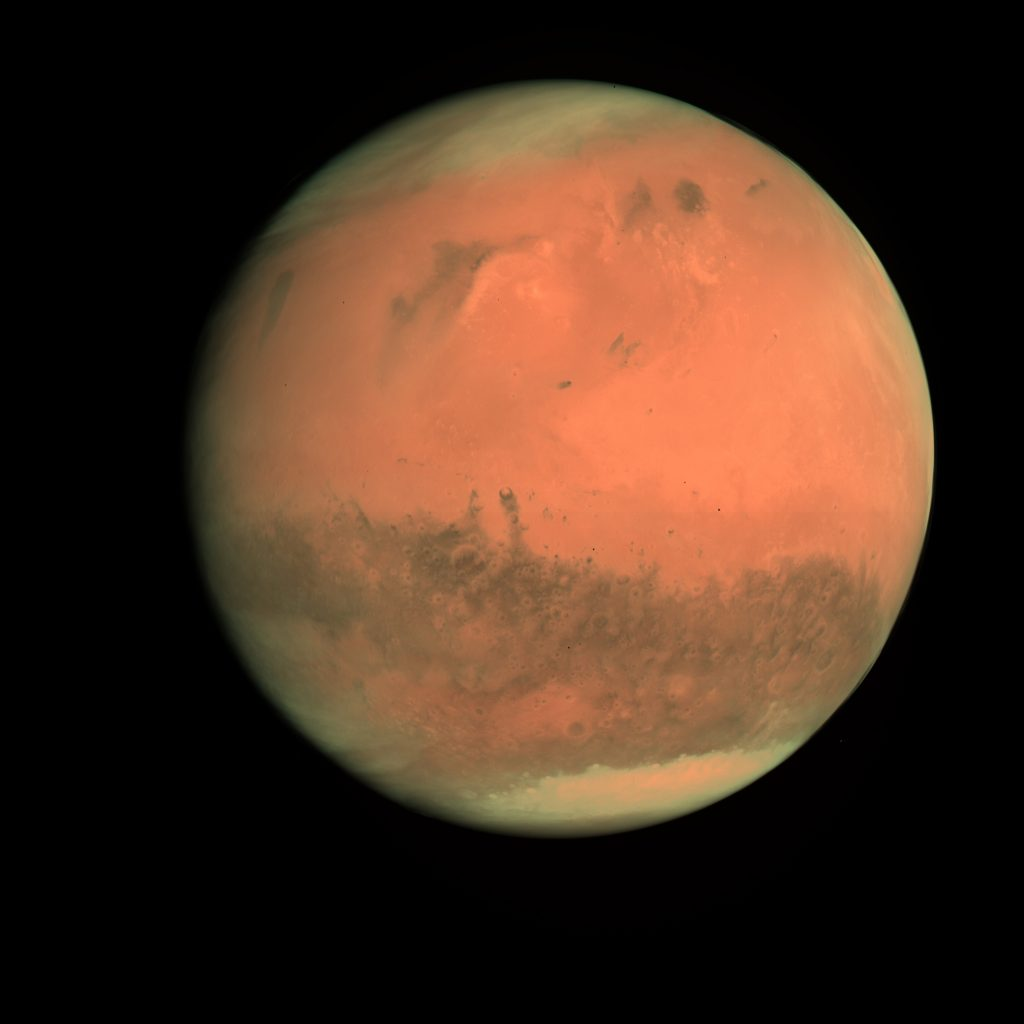
\includegraphics[width=4cm,keepaspectratio]{Image_of_Mars_seen_by_OSIRIS-1024x1024}
    % https://open.esa.int/mars-full-disc-by-rosettas-osiris-camera/
    \caption{
      Mars as seen by Rosetta’s OSIRIS camera (2007). Credit: ESA \& MPS for
      OSIRIS Team MPS/UPD/LAM/IAA/RSSD/INTA/UPM/DASP/IDA, 2007, \href{CC BY-SA
      3.0 IGO}{https://creativecommons.org/licenses/by-sa/3.0/igo/}
    }
  \end{figure}
  \section{Body with $Math$}
  So, I have just been learning about Sch\"odinger Wave Equations or which I
  know remarkably little.
  $${\displaystyle i\hbar {\frac {\partial }{\partial t}}\Psi (\mathbf {r} ,t)=\left[{\frac {-\hbar ^{2}}{2m}}\nabla ^{2}+V(\mathbf {r} ,t)\right]\Psi (\mathbf {r} ,t)}$$
  \section{Body with table}
  \begin{table}[h]
    \centering
      \begin{tabular}{| l c r |}
      \hline
      1 & 2 & 3 \\
      4 & 5 & 6 \\
      7 & 8 & 9 \\
      \hline
    \end{tabular}
    \caption{A simple table}
  \end{table}
  \section{Body with code}
  Sometimes we need some code
  %\[
  %  \displaystyle
  %  F^{(n)}_k := \begin{cases}
  %    0 & \mbox{if } 0 \leq k < n-1 \\
  %    1 & \mbox{if } k = n-1 \\
  %    \sum\limits_{i=k-n}^{(k-1)} F^{(n)}_i & \mbox{otherwise} \\
  %  \end{cases}
  %\]
  \lstinputlisting[
    caption=Haskell implementation of the Fibonacci sequence,
    style=customhs
  ]{src/fib.hs}

  \section{Conclusion}
  With all of this you are now sufficiently informed.
\end{document}
